\documentclass[10pt]{article}
\usepackage[utf8]{inputenc}
\usepackage[T1]{fontenc}
\usepackage{graphicx}
\usepackage[export]{adjustbox}
\graphicspath{ {./images/} }
\usepackage{amsmath}
\usepackage{amsfonts}
\usepackage{amssymb}
\usepackage[version=4]{mhchem}
\usepackage{stmaryrd}
\usepackage{hyperref}
\hypersetup{colorlinks=true, linkcolor=blue, filecolor=magenta, urlcolor=cyan,}
\urlstyle{same}

\title{ome of the United States' fastest-growing and most populous cities are }

\author{}
\date{}


\begin{document}
\maketitle
located in the nation's most arid areas, while some other areas with abundant water are only sparsely populated. For example, Las Vegas, Nevada, located in the Mojave Desert, was among the most rapidly growing U.S. cities from 2000 to 2009 . People flocked to the already-parched city, despite record-low water levels at its primary water source, Lake Mead. Population growth has even led to water stresses in areas previously considered waterrich, such as Atlanta, Georgia.

Water reuse offers an opportunity to significantly expand supplies of freshwater in communities facing water shortages. Coastal areas of the United States, for example, discharge 12 billion gallons of wastewater into estuaries and oceans every day-an amount equivalent to six percent of the country's total daily water use. Reusing this water would directly augment the nation's total water supply.

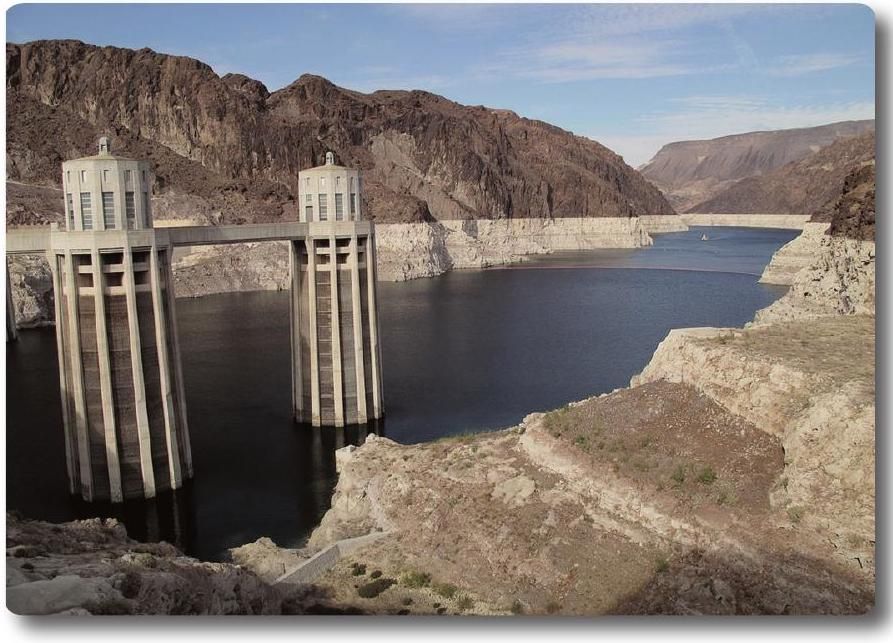
\includegraphics[max width=\textwidth]{2022_11_05_93277ca2de7ec5580550g-01}

Water demands from Las Vegas, Nevada, combined with years of below average precipitation have drained Lake Mead to record-low levels, leaving a white "bathtub ring" 100 feet high.

\section{REUSE, RECYCLE, RECLAIM?}
Water reuse, wastewater reuse, and water recycling all generally mean the same thing: using treated wastewater for a beneficial purpose. The process of treating wastewater prior to reuse is called water reclamation.

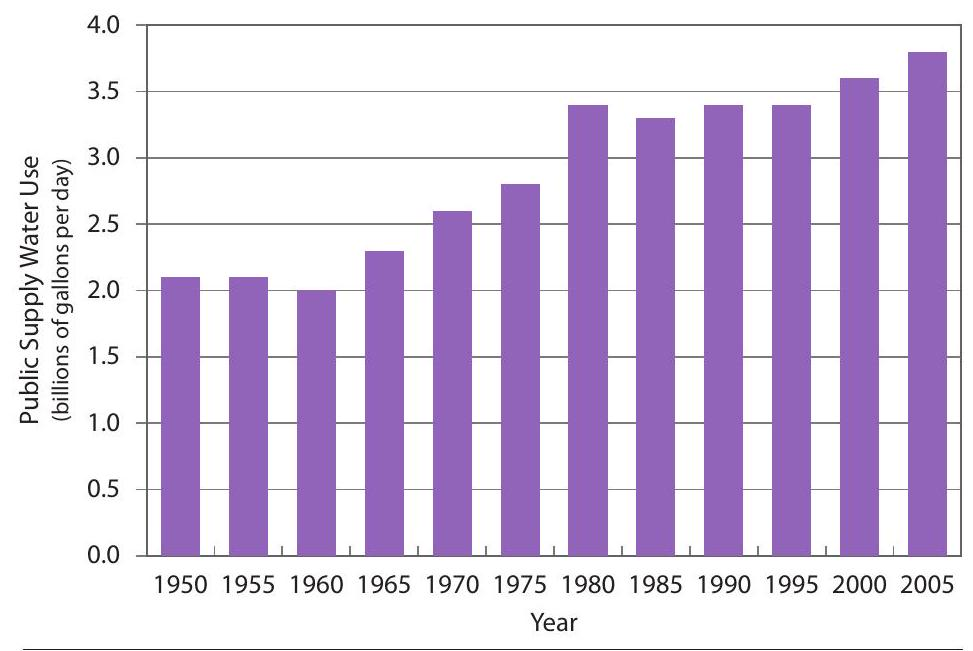
\includegraphics[max width=\textwidth]{2022_11_05_93277ca2de7ec5580550g-01(1)}

Although conservation and improvements in technology have reduced water use for some purposes, such as cooling thermoelectric power plants and other industrial uses, public (or municipal) water use continues to rise, driven in part by expanding and shifting populations. Data from Kenny et al. (2009).

\section{What is Water Reuse?}
n conventional municipal water systems, water from a river, lake, or aquifer is treated to meet drinking water standards before being distributed for all uses. After the water is used, the community's wastewater-the water that flows down the drain or is flushed down the toilet-is treated to remove pollutants before it is discharged into downstream water bodies.

Water reuse is the use of treated wastewater for beneficial purposes, which increases a community's available water supply and makes it more reliable, especially in times of drought.

\section{TYPES OF WATER REUSE}
There are two main types of water reuse projects:

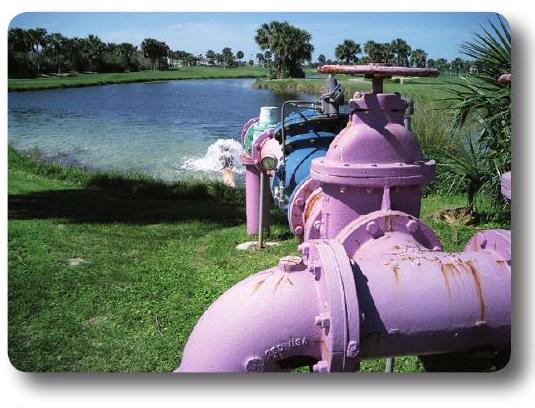
\includegraphics[max width=\textwidth]{2022_11_05_93277ca2de7ec5580550g-02}

In the United States and other countries, purple pipes are used to distinguish nonpotable distribution systems, helping to prevent cross-connections.

\begin{itemize}
  \item Nonpotable reuse projects treat wastewater for specific purposes other than drinking, such as industrial uses, agriculture, or landscape irrigation. Nonpotable reuse could also include the use of reclaimed water to create recreational lakes or to build or replenish wetlands that support wildlife.

  \item Potable reuse projects use highly treated reclaimed wastewater to augment a water supply that is used for drinking and all other purposes.

\end{itemize}
\section{Nonpotable Reuse}
Nonpotable reuse systems typically have lower water quality objectives than potable systems, and the level of treatment varies depending on the end use. Nonpotable reuse usually requires a "dual distribution system"-separate systems of pipes for distributing potable and nonpotable water. Depending on the extent of a community's nonpotable water distribution system, nonpotable reclaimed water can be used for flushing toilets, watering parks or residential lawns, supplying fire hydrants, washing cars and streets, filling decorative fountains, and many other purposes.

The country's oldest dual distribution system is in Grand Canyon Village, Arizona, which has been using reclaimed water for nonpotable uses since 1926. In St. Petersburg, Florida, which began building a large-scale nonpotable reuse system in the 1970s, reclaimed water now satisfies about 40 percent of the city's total water demand, with many of the city's parks, schools, golf courses, residential lawns, fire hydrants, and commercial buildings drawing reclaimed water for nonpotable uses.

In St. Petersburg, Florida, reclaimed water is used for nonpotable purposes such as landscape irrigation.

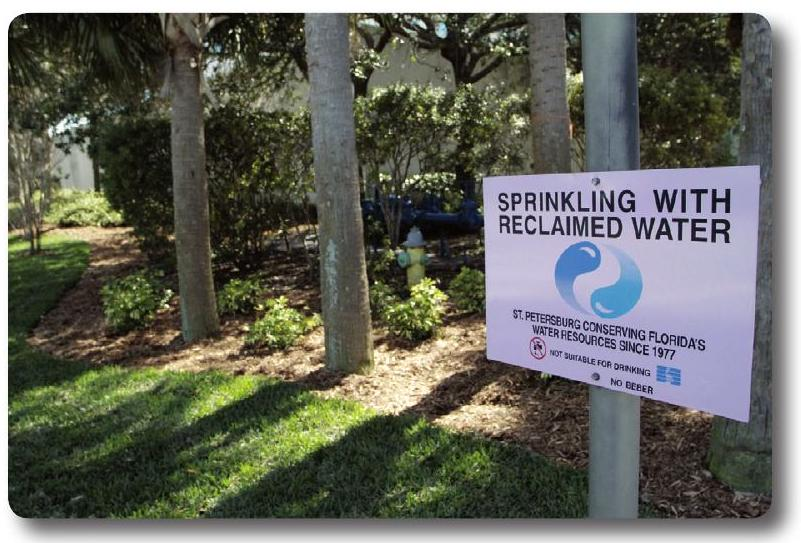
\includegraphics[max width=\textwidth]{2022_11_05_93277ca2de7ec5580550g-02(1)}

\section{Potable Reuse}
Potable reuse systems use advanced treatment processes to remove contaminants from wastewater so that it meets drinking water standards and other appropriate water quality objectives. Typically, the highly treated reclaimed water is then released into a surface water body or aquifer (also called an environmental buffer) before being withdrawn, further treated, blended with other conventional water supply sources, and piped to homes and buildings.

Potable water reuse systems have existed in the United States for 50 years. The Sanitation Districts of Los Angeles County, for example, have been using highly treated reclaimed water to augment Southern California's potable water supply since 1962. Similar systems are in place in other locations in California and in other states, including Virginia, Texas, Georgia, Arizona, and Colorado. About half the nation's potable reuse systems have come on line during the past decade.\\

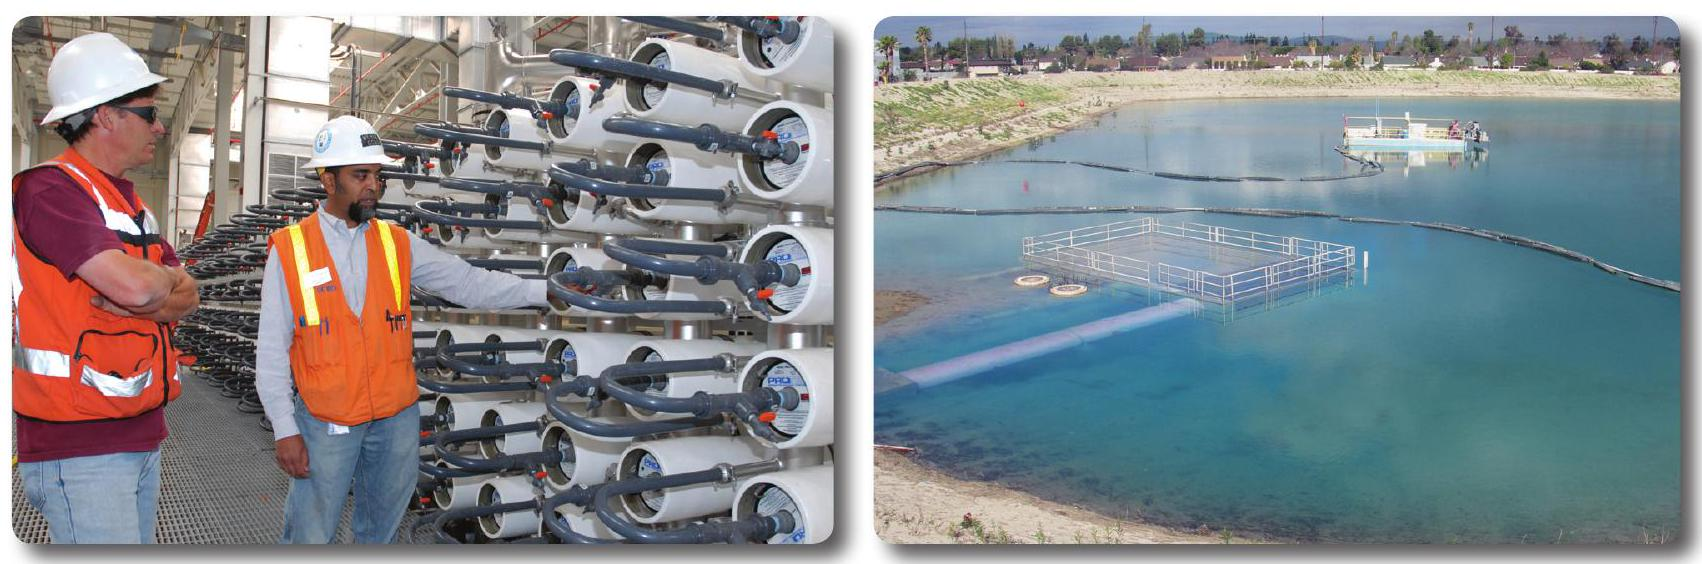
\includegraphics[max width=\textwidth]{2022_11_05_93277ca2de7ec5580550g-03}

Reclaimed water at the Orange County, California, Groundwater Replenishment System is treated by reverse osmosis (left) and other advanced treatment systems before it is either injected into potable water supply aquifers or allowed to percolate into groundwater through infiltration basins (right). Producing 70 million gallons of potable water per day, the project is the country's largest potable water reuse system. It uses wastewater that would otherwise have been discharged into the Pacific Ocean.

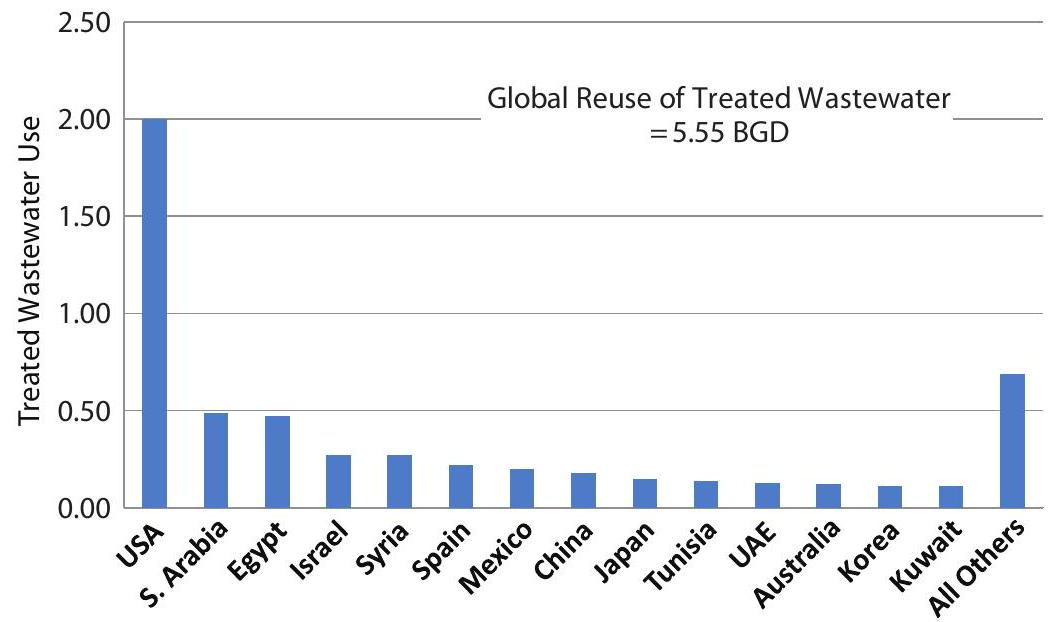
\includegraphics[max width=\textwidth]{2022_11_05_93277ca2de7ec5580550g-03(1)}

According to 2008 estimates, the United States reuses a greater volume of water than any other country (shown here in billions of gallons per day, BGD), and it is ranked thirteenth among countries by per capita water reuse. Qatar and Israel have the highest water reuse per capita. Data from Jiménez and Asano (2008).

\section{De Facto Reuse}
Throughout the United States, some communities may already be reusing wastewater without even realizing it. De facto reuse occurs when a community draws water from a river or reservoir that includes wastewater from upstream communities. De facto reuse is quite common, although it has not been systematically analyzed in the United States in more than 30 years. Since last assessed, de facto reuse has likely increased as expanding cities now discharge more treated wastewater into water sources used by downstream communities. De facto reuse is particularly pronounced in dry periods, when natural water supplies are reduced and wastewater makes up a larger proportion of the water flow.

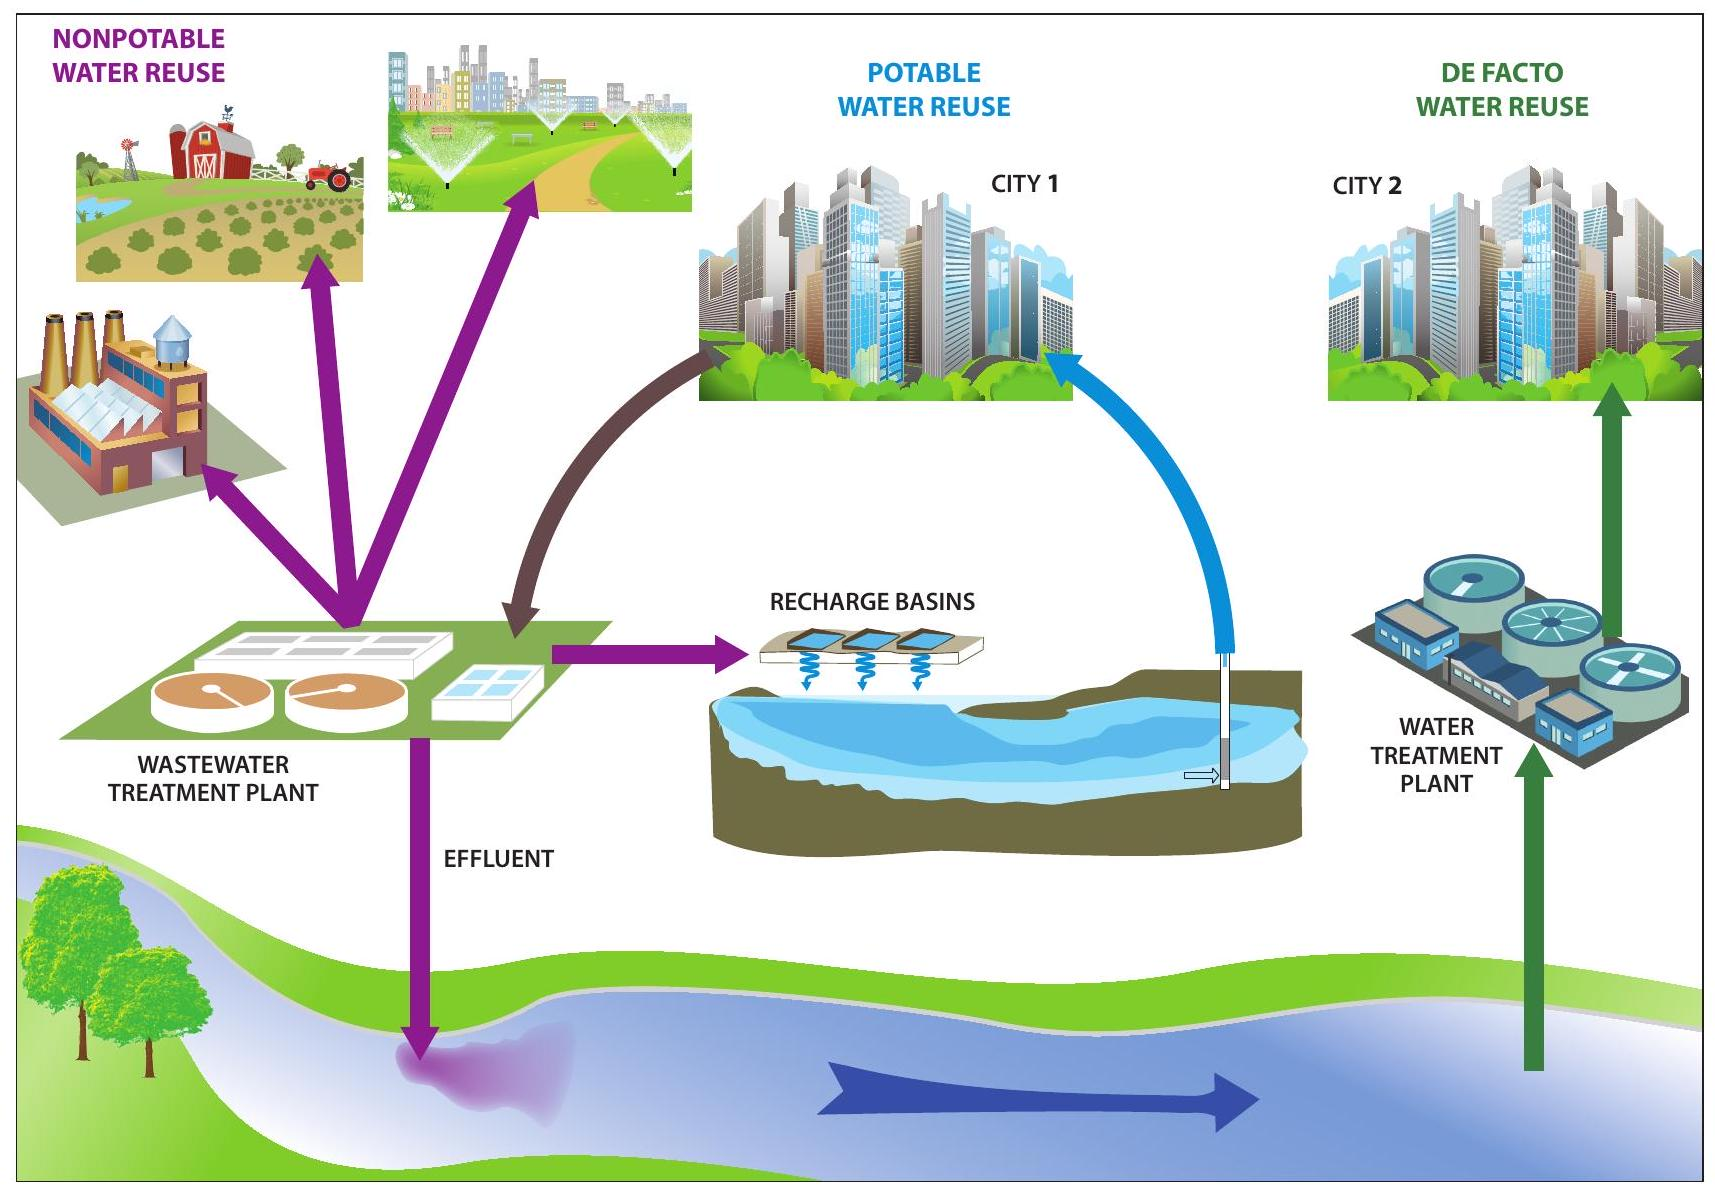
\includegraphics[max width=\textwidth]{2022_11_05_93277ca2de7ec5580550g-04}

The process of treating wastewater and storing, distributing, and using reclaimed water in nonpotable, potable, and defacto reuse. In this schematic, municipal wastewater from City 1 is treated and supplied via a separate distribution system for nonpotable purposes, such as industrial cooling, agriculture, and landscape irrigation. A portion of the city's wastewater receives additional advanced treatment for potable water reuse. The highly treated water is used to recharge groundwater supplies, before it is withdrawn, disinfected, and blended with other drinking water supplies. Some of the treated wastewater effluent from City 1 is also discharged to a nearby river, where it mixes with river water and natural runoff. City 2, a downstream community, withdraws water from the river, treats it to drinking water standards, and uses the water for any purpose. Because the water drawn from the river contains a significant fraction of treated wastewater, this process is called de facto reuse.

\section{CASE STUDY: THE TRINITY RIVER IN TEXAS}
The Trinity River-the main water source for the city of Houston, Texasprovides one documented example of de facto water reuse, although it is by no means a unique situation in the United States. Dallas and Fort Worth draw water from the river's headwaters and discharge their treated wastewater downstream. During summertime and other times when the river's natural flow is reduced, the river consists almost entirely of treated wastewater as it flows away from Dallas and Fort Worth.

After a two-week southward journey, during which natural processes eliminate some trace organic contaminants, the water collects in Lake Livingston-one of Houston's main drinking water reservoirs. There it mixes with rainwater and other water in the reservoir until it is drawn into a drinking water treatment plant and distributed through Houston's taps. Over the course of a year, about half the lake's water is made up of treated wastewater from Dallas and Fort Worth. After treatment, the potable water from the Trinity River meets Environmental Protection Agency drinking water standards.

In one example of de facto water reuse, treated wastewater from Dallas/Fort Worth flows into Lake Livingston, one of Houston's main drinking water reservoirs.

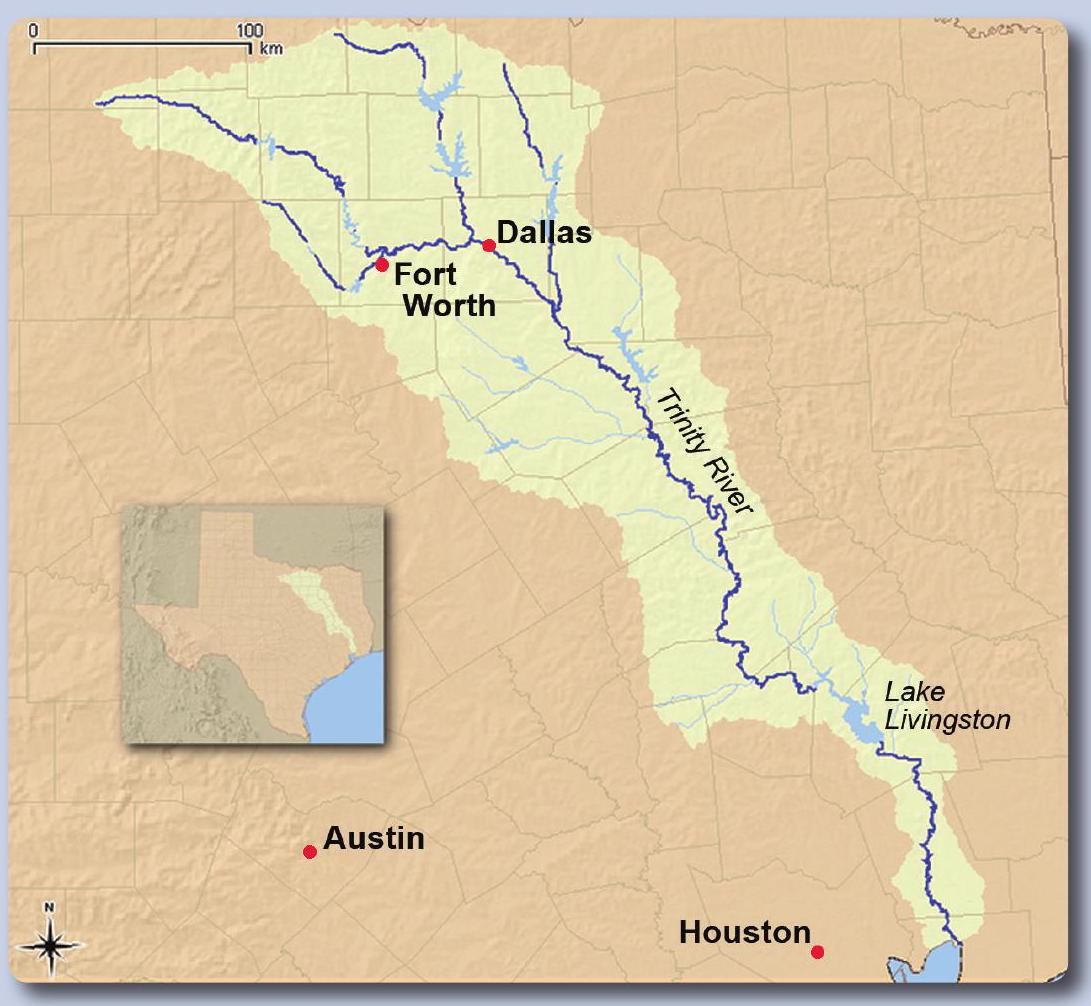
\includegraphics[max width=\textwidth]{2022_11_05_93277ca2de7ec5580550g-05}

\section{Ensuring Water Quality}
community's wastewater typically contains a wide range of microorganisms and chemicals, some of which could be harmful to public health or to ecosystems. Water managers can choose from a portfolio of treatment options to design a wastewater treatment system that reduces contaminants to levels that will be acceptable for the intended uses of the reclaimed water.

Major wastewater contaminants include:

\begin{itemize}
  \item Pathogens. Bacteria, viruses, and other infectious organisms enter wastewater from human excrement and other waste. Viruses with the potential to cause disease are of particular concern for potable reuse because they are very small, can be difficult to eliminate from water, and some can cause infection even at low concentrations.

  \item Nutrients. Municipal wastewaters are rich in nitrogen and phosphorus. Some forms of nitrogen can present a health risk for potable reuse if not properly treated. Excess nutrients can also cause the overgrowth of algae when reclaimed water is used to augment lakes. On the other hand, some nonpotable uses, such as irrigation, are actually enhanced by higher nutrient levels.

  \item Organic chemicals. Pharmaceuticals, natural hormones, household chemicals, and byproducts formed during the treatment process are often present in wastewater. High levels of such chemicals could pose a health risk, particularly for potable uses, unless they are effectively removed or degraded by appropriate water treatment processes.

  \item Other contaminants. Metals and salts are examples of other contaminants that could affect drinking water taste or pose a risk for human health and the environment.

\end{itemize}
Today's advanced analytical methods can detect many contaminants at extremely low levels-but the presence of a contaminant at a low but detectable concentration doesn't always mean that the water poses a significant human health or environmental risk. For example, the risk posed by a particular contaminant varies with the concentration of the contaminant, the intended use of the reclaimed water, and the degree to which people will be exposed to it. Water intended for drinking typically must meet higher quality standards than water intended for nonpotable uses. In addition, different nonpotable uses can have different treatment requirementswater used for industrial cooling might have different quality requirements than those for a lake where swimming is allowed.

Secondary sedimentation basin in a wastewater treatment plant.

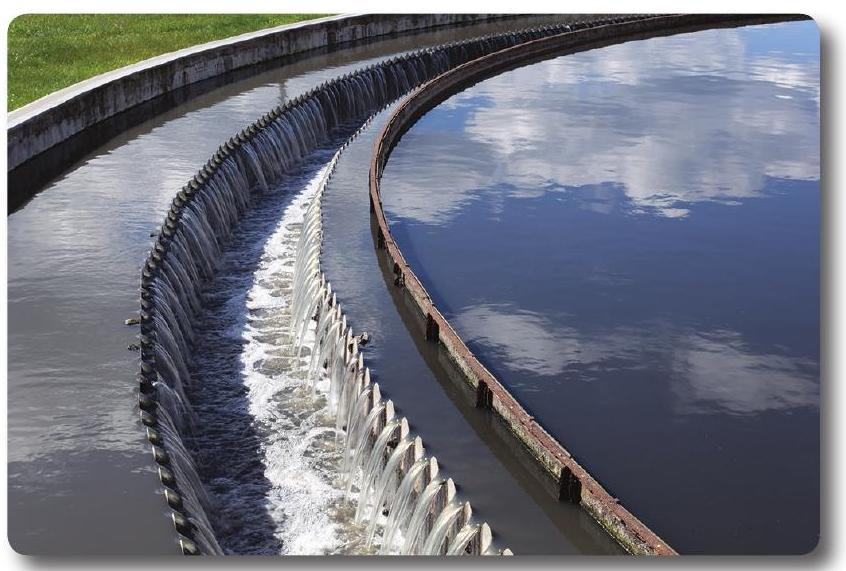
\includegraphics[max width=\textwidth]{2022_11_05_93277ca2de7ec5580550g-06}

\section{TREATMENT TECHNOLOGIES}
There are a number of technologies available for treating wastewater intended for reuse, many of which can be used in combination. To choose the appropriate combination of treatment options, water managers must consider the specific contaminants that are of concern, the intended use of the water, costs, and other factors such as energy use or waste disposal options.

The National Research Council report reviewed options for ensuring water quality in water reuse projects. Because protecting public health is of utmost importance for any drinking water system, the report's authoring committee recommended potable water reuse systems include several redundant treatment elements to strengthen the reliability of the system.

In addition to redundant treatment processes, the committee recommended that water reuse systems incorporate plans for monitoring water quality and quickly responding to problems caused by equipment malfunctions, operator error, or changes in the quantity or quality of incoming wastewater. For nonpotable reuse systems, it is also important to prevent drinking water contamination from the inadvertent cross-connection of nonpotable water and potable water pipes.

Treatment processes commonly used in water reclamation. At each stage of processing, several treatment options are available. Water managers can choose one or more of these options to create a process that will treat water to the quality needed for its intended use. Water treatment begins with preliminary and primary treatment, which targets suspended and particulate matter,

followed by secondary treatment to remove biodegradable organic carbon. Water managers can then choose to proceed to advanced treatment, which provides additional removal of nutrients, trace organic chemicals, and suspended solids. Engineered natural processes allow reclaimed water to blend with water from other sources and provide additional natural treatment to further remove contaminants from the water.

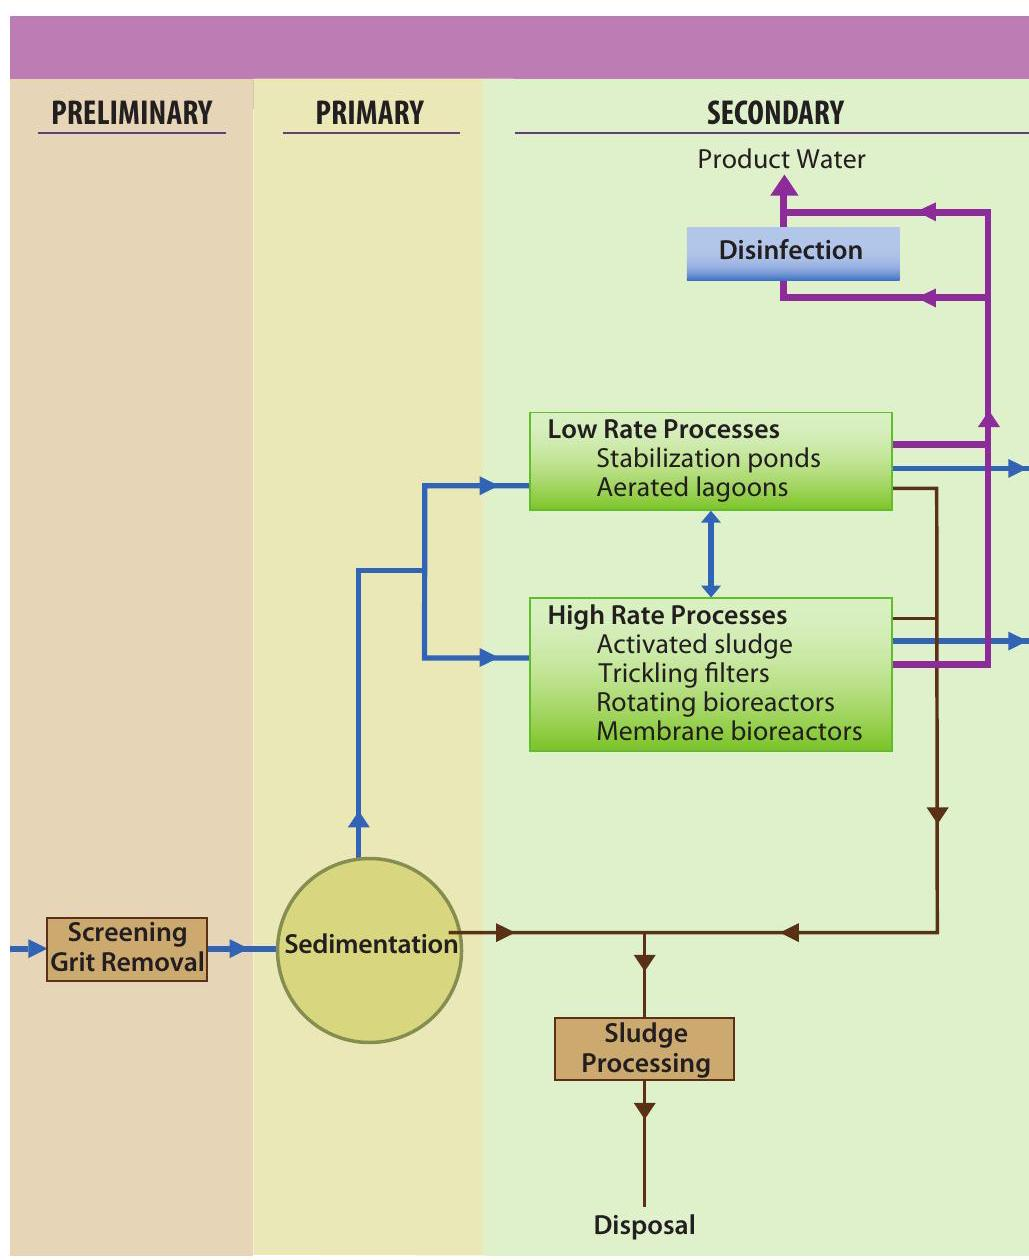
\includegraphics[max width=\textwidth]{2022_11_05_93277ca2de7ec5580550g-07}

\section{THE EVOLVING ROLE OF ENVIRONMENTAL BUFFERS}
In many potable reuse systems, environmental buffers such as aquifers, lakes, or wetlands serve a number of purposes. They are used to hold reclaimed water to provide additional time before it is introduced into a drinking water system and to allow it to blend with water from other sources. Environmental buffers may also provide additional natural treatment to further remove contaminants from the water, and they create psychological distance between the water's source (treated wastewater) and its destination (drinking water) by incorporating natural environments into the process.

Until recently, environmental buffers were considered a core element of all potable reuse projects. However, the National Research Council committee concluded that environmental buffers do not provide any water quality services that cannot also be provided by the use of engineered processes, such as advanced treatment and constructed storage facilities. Although environmental buffers remain useful elements of water treatment systems that should be considered alongside other options, they are not essential elements to reach water quality goals. Since 2010, several potable reuse projects have been developed or proposed that do not incorporate environmental buffers.

\section{Engineered Unit Processes and Operation}
ADVANCED

ENGINEERED NATURAL PROCESSES

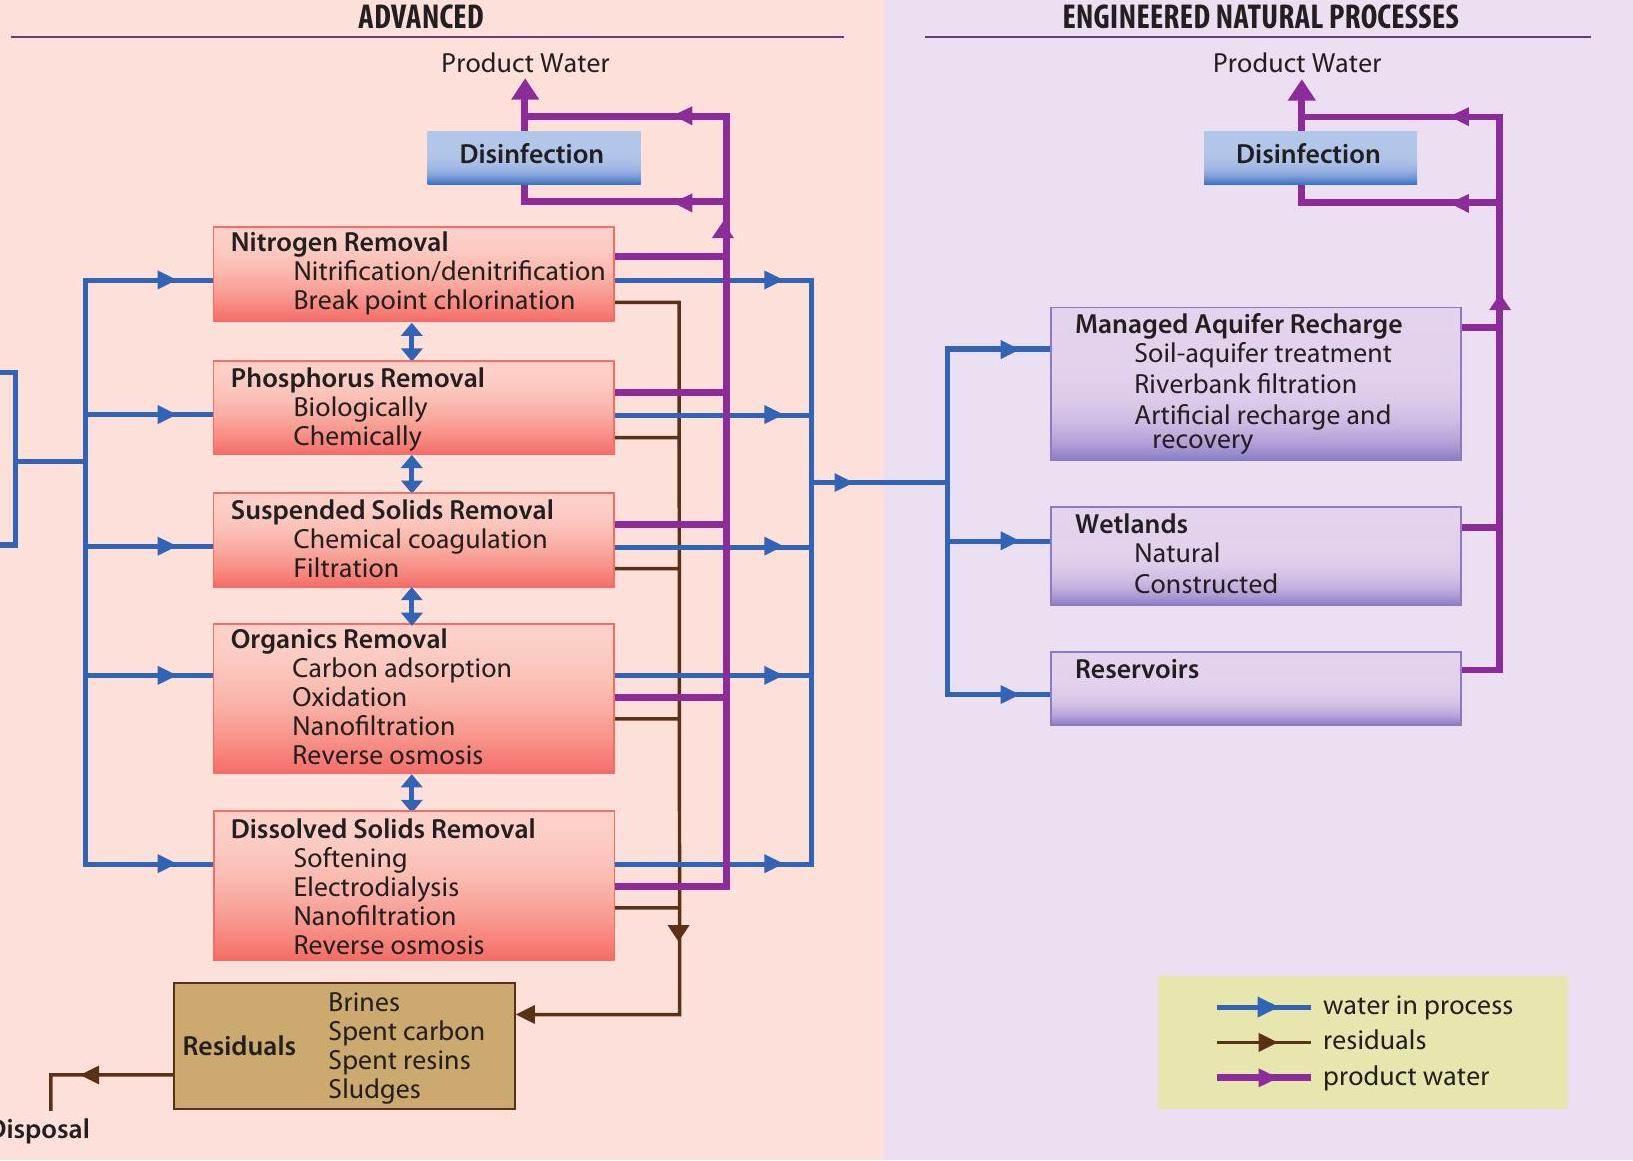
\includegraphics[max width=\textwidth]{2022_11_05_93277ca2de7ec5580550g-08}

\section{Assessing the Risks of Potable Water Reuse in Context}
he committee that wrote the National Research Council report conducted an analysis that compares the estimated risks of drinking water from two potable reuse projects to a de facto reuse scenario in which five percent of the source water comes from wastewater discharged upstream after secondary treatment. The assumed de facto reuse conditions of scenario 1 are likely typical in many places and are generally perceived as safe. In scenario 2, treated wastewater is allowed to filter slowly through surface soils into an aquifer (also called soil aquifer treatment) before potable reuse. In scenario 3 , advanced treatment techniques including microfiltration, reverse osmosis, and advanced oxidation are employed before the water is injected into an aquifer and used as a source of drinking water.

The analysis compared the risks of exposure to four pathogens (adenovirus, norovirus, Salmonella, and Cryptosporidium) and 24 chemical contaminants including pharmaceuticals,

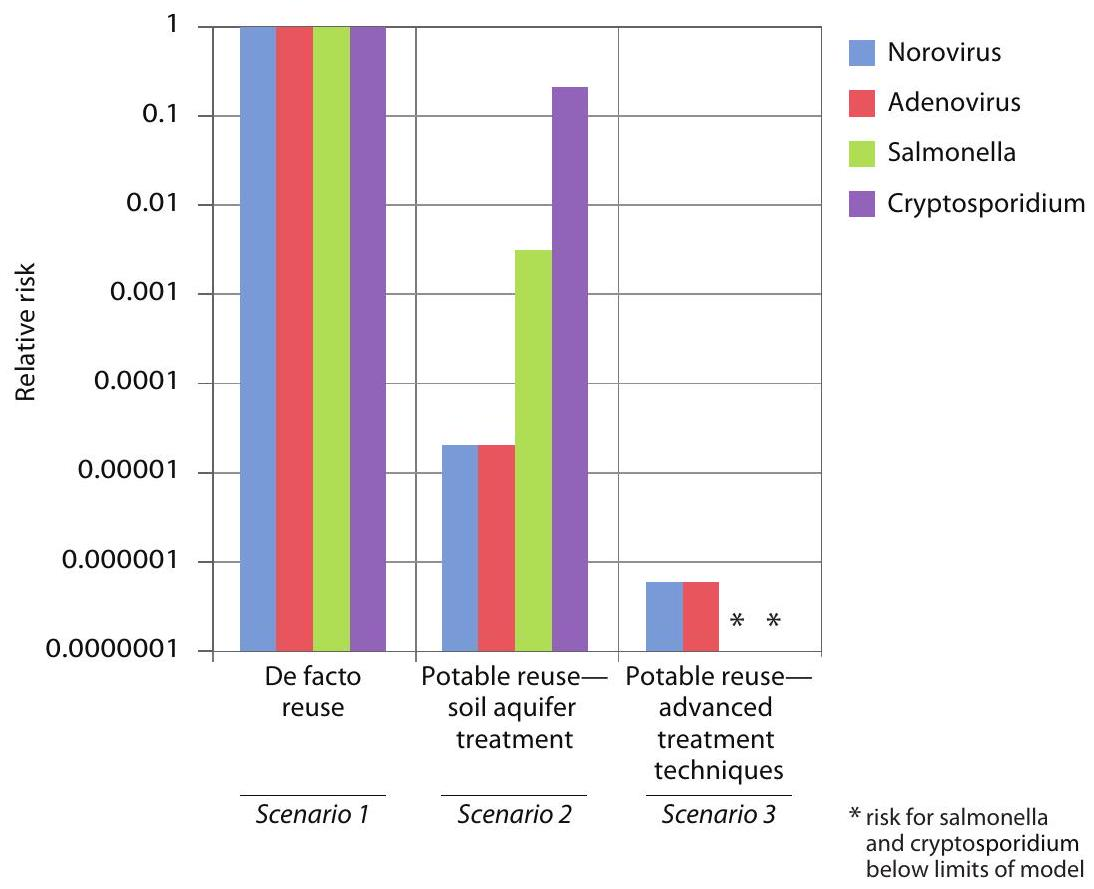
\includegraphics[max width=\textwidth]{2022_11_05_93277ca2de7ec5580550g-09}

Relative risk, shown on a logarithmic scale, posed by selected pathogens in a typical de facto reuse scenario (1), compared to two potable reuse scenarios $(2,3)$. The smaller the number, the lower the relative risk. For example in Scenario 2 , the risk of illness due to Salmonella is estimated to be less than 1/100th of the risk due to Salmonella in Scenario 1. Overall, the results indicate the risk of exposure to these pathogens from drinking reclaimed water does not appear to be any higher than the risk experienced in at least some current drinking water treatment systems. personal care products, natural hormones, industrial chemicals, and byproducts from water disinfection processes.

The results suggest that the risk of exposure to certain microbial and chemical contaminants from drinking reclaimed water does not appear to be any higher than the risk experienced in at least some current drinking water treatment systems-and may, in fact, be orders of magnitude lower.

The analysis revealed that carefully planned potable water reuse projects should be able to provide a level of protection from waterborne illness and chemical contaminants comparable toand, in some cases, better than-the level of protection the public

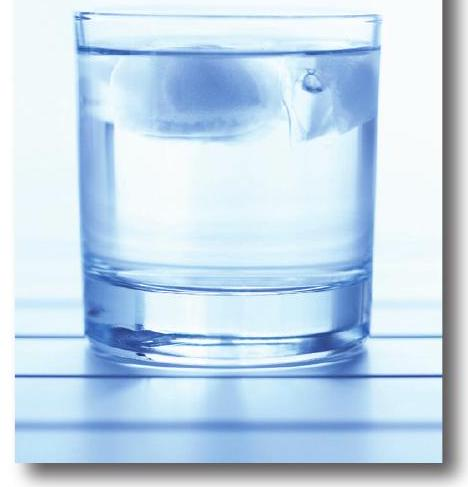
\includegraphics[max width=\textwidth]{2022_11_05_93277ca2de7ec5580550g-10}\\
experiences in many drinking water supplies across the nation. However, the committee pointed out that the analysis was presented as an example and should not be used to endorse certain treatment schemes or to determine the risk at any particular site without site-specific analysis.

\section{Costs of Water Reuse Projects}
nvesting in a water reuse system is a complex decision with both costs and benefits that extend many years into the future. Generally, water reuse is more expensive than drawing water from a natural freshwater source, but less expensive than seawater desalination. In many cases, lower-cost water sources are already being used, so the cost of water reuse should be compared with the cost of any available new water sources. The costs of water reuse vary greatly from place to place depending on location, water quality requirements, treatment methods, distribution system needs, energy costs, interest rates, subsidies, and many other factors.

Potable reuse systems can be more or less expensive than nonpotable reuse systems. Nonpotable reuse may require less treatment, depending on the intended use of the reclaimed water, and can also reduce the peak demand on a potable system, which can be a huge factor on water use in arid locations. However, nonpotable reuse also typically requires a separate piping system, which can be a significant expense depending on where and how far nonpotable water must be distributed.

Water managers should also consider non-monetary costs and benefits of reuse projects, such as increased water supply reliability in times of drought, greenhouse gas emissions, and ecological impacts, to determine the most socially, environmentally, and economically feasible water supply option for their community.

\section{Public Preferences and Acceptability}
he public is a major stakeholder in any water management decision, and community members often play an important role in making decisions about water reuse projects. As with any water project, the success or failure of a proposed reuse project can ride on public perceptions of how the project relates to public health, public finance, taste and aesthetics, land use, environmental protection, and economic growth.

Humans have a natural revulsion to water that is perceived to be contaminated, and sometimes that feeling can translate into opposition to reusing treated wastewater, even when reclaimed water is shown to be of high quality. In some cases, people may even prefer lowerquality water from a source perceived as "natural" over higher-quality water coming from an advanced wastewater treatment facility. Reclaimed water's history as wastewater causes a psychological barrier for many people that can be hard to overcome.

However, when communities are actively engaged in discussions about water reuse, the technologies and science behind it, and the overall context of water management, both the public and water managers are better equipped to engage in meaningful dialogue.

In Redwood City, California, for example, a proposed water reclamation project was temporarily stalled by opposition from a small citizens' group in 2002. In response, a task force was established that brought the two sides together to discuss the project, review reliable sources of information, and weigh alternative options. A modified reuse project was eventually approved that was widely supported by the community. As the Redwood City experience demonstrates, frequent and open communication among water managers, citizens, and governments can be critical for communities to address the concerns of the public and make informed decisions about water reuse.

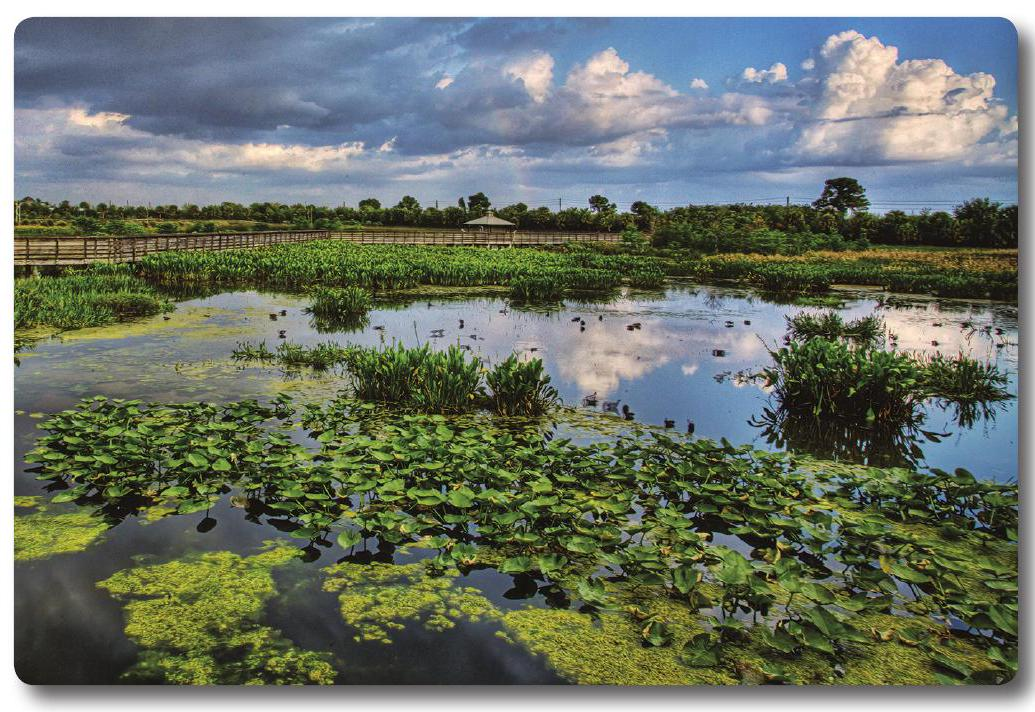
\includegraphics[max width=\textwidth]{2022_11_05_93277ca2de7ec5580550g-11}

Green Cay Wetlands in Palm Beach County, Florida, provide additional nutrient removal for several million gallons of highly treated wastewater per day. The water then recharges groundwater supplies. Environmental buffers, such as this one, have been important for gaining public support in past potable reuse projects. This booklet is based on Water Reuse: Expanding the Nation's Water Supply through Reuse of Municipal Wastewater by the Committee on the Assessment of Water Reuse as an Approach to Meeting Future Water Supply Needs. The report was supported by funding from the Environmental Protection Agency, the U.S. Bureau of Reclamation, the National Science Foundation, the National Water Research Institute, the Centers for Disease Control and Prevention, the Water Research Foundation, Orange County Water District, Orange County Sanitation District, Los Angeles Department of Water and Power, Irvine Ranch Water District, West Basin Water District, Inland Empire Utilities Agency, Metropolitan Water District of Southern California, Los Angeles County Sanitation Districts, and the Monterey Regional Water Pollution Control Agency. Production of this

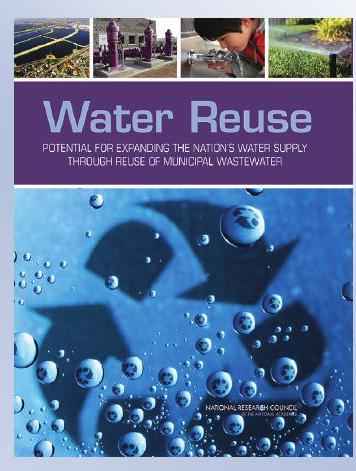
\includegraphics[max width=\textwidth]{2022_11_05_93277ca2de7ec5580550g-12}\\
booklet was supported by additional funding from the U.S. Bureau of Reclamation.

For more information relating to the report, visit: \href{http://nas-sites.org/waterreuse}{http://nas-sites.org/waterreuse}


\includegraphics[max width=\textwidth]{2022_11_05_93277ca2de7ec5580550g-12(1)}

Committee on the Assessment of Water Reuse as an Approach to Meeting Future Water Supply Needs

Rhodes R. Trussell (Chair), Trussell Technologies, Pasadena; Henry A. Anderson, Wisconsin Division of Public Health; Edmund G. Archuleta, El Paso Water Utilities PSB, Texas; James Crook, Environmental Engineering Consultant, Norwell, Massachusetts; Jörg E. Drewes, Colorado School of Mines; Denise D. Fort, University of New Mexico, Albuquerque; Charles N. Haas, Drexel University, Philadelphia; Brent M. Haddad, University of California, Santa Cruz; Duane B. Huggett, University of North Texas, Denton; Sunny Jiang, University of California, Irvine; David L. Sedlak, University of California, Berkeley; Shane A. Snyder, University of Arizona, Tucson; Margaret H. Whittaker, ToxServices LLC, Washington, D.C.; Dale Whittington, University of North Carolina, Chapel Hill; Stephanie E. Johnson (Study Director), Sarah E. Brennan (Program Assistant, from July 2010), Stephen Russell (Program Assistant, until July 2010), National Research Council.

Data Sources for Charts

p.2-Kenny, J., N. Barber, S. Hutson, K. Linsey, J. Lovelace, and M. Maupin. 2009. Estimated Use of Water in the United States in 2005. USGS Circular 1344. Reston, VA: U.S. Geological Survey.

p.3-Jiménez, B., and T. Asano. 2008. Water reclamation and reuse around the world. In B. Jimenéz and T. Asano, eds., Water Reuse: An International Survey of Current Practice, Issues and Needs. London: IWA Publishing, pp. 3-26.

\section{Credits}
\href{mailto:p.1-@iStockphoto.com}{p.1-@iStockphoto.com}/Jitalia17. p.3-(top) Mr Noded; (bottom) Dennis MacDonald/World of Stock.

p.4-Orange County Water District, Orange County, California. p.6-Kuru via Wikipedia.

p.7-Jonutis/shutterstock. p.12-@2011 Kim Y. Seng.

(C) 2012 National Academy of Sciences.

\section{About the National Academies}
The National Academies—the National Academy of Sciences, National Academy of Engineering, Institute of Medicine, and the National Research Council—provide a public service by working outside the framework of government to ensure independent advice on matters of science, technology, and medicine. They enlist committees of the nation's top scientists, engineers, and other experts-all of whom volunteer their time to study specific concerns. The results of these deliberations are authoritative, peer-reviewed reports that have inspired some of the nation's most significant efforts to improve the health, education, and welfare of the population.


\end{document}